% Options for packages loaded elsewhere
\PassOptionsToPackage{unicode}{hyperref}
\PassOptionsToPackage{hyphens}{url}
%
\documentclass[
  a4paper,
  11pt,
  twocolumn]{article}
\usepackage{amsmath,amssymb}
\usepackage{lmodern}
\usepackage{iftex}
\ifPDFTeX
  \usepackage[T1]{fontenc}
  \usepackage[utf8]{inputenc}
  \usepackage{textcomp} % provide euro and other symbols
\else % if luatex or xetex
  \usepackage{unicode-math}
  \defaultfontfeatures{Scale=MatchLowercase}
  \defaultfontfeatures[\rmfamily]{Ligatures=TeX,Scale=1}
\fi
% Use upquote if available, for straight quotes in verbatim environments
\IfFileExists{upquote.sty}{\usepackage{upquote}}{}
\IfFileExists{microtype.sty}{% use microtype if available
  \usepackage[]{microtype}
  \UseMicrotypeSet[protrusion]{basicmath} % disable protrusion for tt fonts
}{}
\makeatletter
\@ifundefined{KOMAClassName}{% if non-KOMA class
  \IfFileExists{parskip.sty}{%
    \usepackage{parskip}
  }{% else
    \setlength{\parindent}{0pt}
    \setlength{\parskip}{6pt plus 2pt minus 1pt}}
}{% if KOMA class
  \KOMAoptions{parskip=half}}
\makeatother
\usepackage{xcolor}
\IfFileExists{xurl.sty}{\usepackage{xurl}}{} % add URL line breaks if available
\IfFileExists{bookmark.sty}{\usepackage{bookmark}}{\usepackage{hyperref}}
\hypersetup{
  hidelinks,
  pdfcreator={LaTeX via pandoc}}
\urlstyle{same} % disable monospaced font for URLs
\usepackage{graphicx}
\makeatletter
\def\maxwidth{\ifdim\Gin@nat@width>\linewidth\linewidth\else\Gin@nat@width\fi}
\def\maxheight{\ifdim\Gin@nat@height>\textheight\textheight\else\Gin@nat@height\fi}
\makeatother
% Scale images if necessary, so that they will not overflow the page
% margins by default, and it is still possible to overwrite the defaults
% using explicit options in \includegraphics[width, height, ...]{}
\setkeys{Gin}{width=\maxwidth,height=\maxheight,keepaspectratio}
% Set default figure placement to htbp
\makeatletter
\def\fps@figure{htbp}
\makeatother
\setlength{\emergencystretch}{3em} % prevent overfull lines
\providecommand{\tightlist}{%
  \setlength{\itemsep}{0pt}\setlength{\parskip}{0pt}}
\setcounter{secnumdepth}{5}
%------------------------------------------------------------------------------%
% PAPER TEMPLATE FOR ICPHS 2019 MELBOURNE                                      %
%                                                                              %
% Original template downloaded from:                                           %
% http://www.icphs2019.org/call-for-papers/                                    %
%                                                                              %
% Reformatted to work with Rmarkdown and R by:                                 %
% Joseph V. Casillas | Rutgers Univesity | 6/6/2018                            %
%                                                                              %
% Available for download at:                                                   %
% https://github.com/jvcasillas/icphs2019_rmd_template                         %
%------------------------------------------------------------------------------%



% Packages
\usepackage{./includes/tex/icphs2019}
\usepackage{metalogo} 
\usepackage{epstopdf}
\usepackage{tipa}

% Links and urls must be black
\hypersetup{urlcolor=black, citecolor=black, linkcolor=black}


% Packages removed from icphs2019.sty because of conflicts
% They have been added to the .Rmd yaml front matter
% \usepackage[latin1]{inputenc}
% \usepackage[T1]{fontenc}
% \usepackage[leqno,fleqn]{amsmath}
\usepackage[T1]{fontenc}
\ifLuaTeX
  \usepackage{selnolig}  % disable illegal ligatures
\fi

\author{}
\date{\vspace{-2.5em}}

\begin{document}

\title{A simulated analysis of repeated measures in VOT: we need more tokens!}
\author{Kyle Parrish}
\organization{Rutgers University}
\email{kyle.parrish@rutgers.edu}


\maketitle

\begin{abstract}
In speech research, studies often make use of repeated measures, in which multiple tokens per condition are taken from the same participant and incorporate them into multilevel models. For instance, in VOT studies, researchers often elicit productions of stop consonants from multiple words produced by the same participant. It is unclear, however, how many repetitions of the same segment are necessary and how researchers go about choosing this number. The present study used reported data from previous literature to simulate an underlying distribution of 1000 points for each stop consonant (/p/, /t/, /k/, /b/, /d/, /g/) in order to determine how many of these tokens were necessary so that the random sample would be practically equivalent sample to the full simulated distribution.The results suggest that at least 15 tokens are necessary for all 6 stop consonants to achieve a practically equivalent sample (equivalence bounds d = +/- .4).
\end{abstract}

\keywords{Repeated Measures, VOT, simulation.}


\section{Introduction}

Linguistic and psychological research of human subjects is often
concerned with characterizing the behavior of a participant in distinct
experimental conditions. It is generally agreed that, in most cases, it
is necessary for experimenters to collect a sample of participants from
a hypothetical underlying distribution, since the resources involved
make it impossible to collect data from every possible subject meeting
some given group criteria. For example, if one wanted to determine how
the segment /a/ is produced in American English, it would likely not be
feasible to collect tokens of /a/ from every American English speaker.
Rather, the researcher collects a particular number of participants
which serves as a random sample from a hypothetical underlying
distribution. In general, the number of participants necessary for a
faithful sample are determined by power analysis, where a researcher
specifies an effect size, power level, significant threshold and finds
the minimum number of participants needed to reliably find that effect.

In addition to knowing the appropriate number of participants for a
study, the number of repetitions of a particular sound by each of those
participants is another factor which has received much less attention.
Following the same logic as sampling from a distribution of
participants, it is also the case that researchers cannot collect all
productions of a given sound from a subject, and must collect a sample.
While most studies in speech research utilize repeated measures, it is
unclear how the number of productions of a given segment are justified.

The quantity of repeated measures has varied in the literature. For
instance, in their tutorial for multilevel models, Baayen and colleagues
\cite{baayen2008mixed} simulated 3 tokens per condition in their
multilevel model. Although their data set was simulated to demonstrate
the nested structure of data and that data points from the same
individual are not independent, the decision of 3 repetitions per token
in this paper appears to be arbitrary.

In speech research, the quantity of repeated measures has also varied.
Given their abundance, VOT studies provide a good example of the
variation in repeated measures in speech research, and are the focus of
the present paper. To investigate the use of repeated measures in recent
VOT studies, a brief analysis of relevant studies in VOT was carried out
focusing on the Journal of Phonetics. Using their website, a search for
the term ``VOT production'' sorted by relevance revealed that the six
most relevant articles range from 3 to 50 tokens per segment and
condition \cite{fish2017infant}, \cite{antoniou2011inter},
\cite{olson2013bilingual}, \cite{hussain2018typological},
\cite{gorba2022acquisition}, \cite{chodroff2017structure}. To be clear,
these studies ranged in how they divided conditions. In some cases, the
all stop consonants were presented in a single vocalic context
\cite{olson2013bilingual}, while others elicited stops with many vowel
sounds \cite{chodroff2017structure}. Here, the focus of repeated
measures is the quantity of tokens per segment per language (in a
bilingual context), thus the same stop in the same language, but in a
different vocalic context were counted as belonging to the same
condition. For example, Chodroff and Wilson \cite{chodroff2017structure}
analyzed all 6 stops in American English and included 5 repetitions of
each stop in 10 vocalic contexts, for a total of 50 productions of each
stop per participant. Table \ref{tab:decibel} shows a breakdown of the
top studies returned by the search and their tokens per condition.

\begin{table}[!ht]
  \caption{Most relevant studies by filter in the Journal of Phonetics}
  \label{tab:decibel}
  \begin{center}
  \begin{tabular}{|c|c|}
  \hline
  \rowcolor[gray]{.75}
  Study    & Repetitions \\
  \hline
  $Olson\ (2013)$   & $3$    \\
  $Antoniou\ (2011)$    & $4$      \\
  $Hussain\ 2018$   & $5$     \\
  $Fish\ (2017)$  & $9-12$     \\
  $Gorba\  \&\ Cebrian\ (2022)$    & $10$      \\
  $Chodroff\ \&\ Wilson\ (2017)$   & $45-50$     \\
  \hline
  \end{tabular}
  \end{center}
\end{table}

The source of the variation in the number of repeated measures in the
literature is unclear, but could be made more consistent by carrying out
a power analysis, similarly to how sample size is justified. The power
of a sample refers to the probability of detecting an effect when it
exists \cite{cohen1992statistical}. A power analysis consists of four
parts, an significance threshold (typically .05), a power level
(typically .8), a sample size and an effect size. Given three of these
four, a power analysis calculates the missing number. For example, with
the significance threshold at .05 and the power level of .8, a power
analysis reveals that about 80 participants are needed per group to
reliably detect a small effect (Cohen's D = .4). Although speech
research is often concerned with finding differences in groups or
conditions, it is also possible and useful to conduct a power analysis
to determine the probability of detecting practical equivalence within a
particular effect size. In this case, a threshold for practical
equivalence can be specified, along with a number of samples and
significance threshold. As a result, the power analyses of the present
study refer to the probability of detecting practical equivalence,
rather than a particular effect size, when it exists.

The present study implements this approach using the reported means and
standard deviations in Chodroff and Wilson (2017)
\cite{chodroff2017structure}. The present study carries out several
power analyses on large simulated data sets of a 6 stop consonants in
English to determine how many tokens are necessary to consistently
generate a sample that reliably falls within a small effect size of the
simulated underlying distribution.\\
That is, if we consider the speaker to be producing VOT from an
underlying distribution of possible values, we can analyze how many
samples from that distribution are needed to achieve a particular level
of precision when we characterize an individual's stop production. In
particular, the present study is guided by the following research
question:

RQ1: For each of the 6 stop consonants in English, how many tokens are
necessary to produce a sample that is practically equivalent (falls
within Cohen's d = +/- .4 on the test of equivalence p \textgreater{}
.05) to the underlying sampling distribution (a simulated data set of
1000 points).

It was predicted that, just like power analyses of needed participants,
that more samples would be associated with higher power.

\section{Methods}

All data used for the present study were simulated using the rnorm
function in R. First, for each stop (/p/,/t/,/k/,/b/,/d/,/g/), an
underlying distribution of 1000 points each was generated. The means and
standard deviations of each distribution came from the from the
literature (see Table \ref{tab:stim}) \cite{chodroff2017structure} for
all 6 top consonants. This underlying distribution was generated to
serve as a the representation of all possible realizations of a given
consonant which were each equally probable to be produced by a given
individual, although the true mean and standard deviation of this
distribution will never be known.

\begin{table}[!ht]
  \caption{Means and Standard Deviations for each Stop Consonant in American English from Chodroff \& Wilson (2017)}
  \label{tab:stim}
  \begin{center}
  \begin{tabular}{|c|c|}
  \hline
  \rowcolor[gray]{.75}
  Segment    & Mean (SD) \\
  \hline
  $/p/$    & $89 (27)$      \\
  $/t/$    & $98 (28)$      \\
  $/k/$   & $99 (24)$     \\
  $/b/$   & $13 (5)$    \\
  $/d/$   & $21 (7)$     \\
  $/g/$  & $28 (10)$     \\
  \hline
  \end{tabular}
  \end{center}
\end{table}

Then, using the generated underlying distribution, the sample\_n
function in R was used in a loop function to randomly select a given
number of tokens from the total of 1000. The sample sizes analyzed were
6, 10, 12, 15, and 18, which were looped 100 times each. For example, if
the sample size was 6, then the function chose 6 random rows of the
total of 1000 per iteration. Following the selection of the 6 random
tokens, a test of equivalence \cite{lakens2017equivalence}, and a
Welch's T-test were carried out between the random sample (e.g., the 6
random tokens of that iteration) and underlying distribution (all 1000
tokens). Overall, this process generated 30000 total data points, given
that 100 simulations were carried out per participant (10) per sample
size (5) in each of the segments (6).

The test of equivalence used equivalence bounds of +/- d = .4, or a less
than a small effect in language research based on a recent study
\cite{plonsky2014big}. In other words, the present study considered a
random sample from a participant's greater distribution to be
practically equivalent when the difference between the sample and all
their productions was less that a small effect. That is, although there
were still differences detected, the present study assumed them to be
caused by noise, rather than a meaningful difference when the effect
size was less than .4. The data were coded for whether or not the test
of equivalence or t-test were was significant for a given iteration (1
for yes/0 for no). Data for effect sizes and mean differences were also
stored per iteration, although this information is not reported in the
present paper.

\section{Results}

Figure 1 shows the percentage of practically equivalent results in each
sample size for each segment. The figure suggests that at least 15
samples of a given segment are needed to achieve a sample that is within
d = +/- .4 at least 80 percent of the time, while 18 would be best. 6
tokens per segment was the least successful at producing a practically
equivalent sample, as all segments were practically equivalent less than
50 percent of the time. Table \ref{tab:nums} reports the percentage of
significant tests of equivalence for each segment and each sample size.
Again, for each segment, at least 15 tokens are necessary to produce a
practically equivalent sample at least 80 percent of the time.

\begin{figure}[!ht]
  \caption{Quantity of practically equivalent instances per sample size}
  \label{fig:stim}
  \begin{center}
  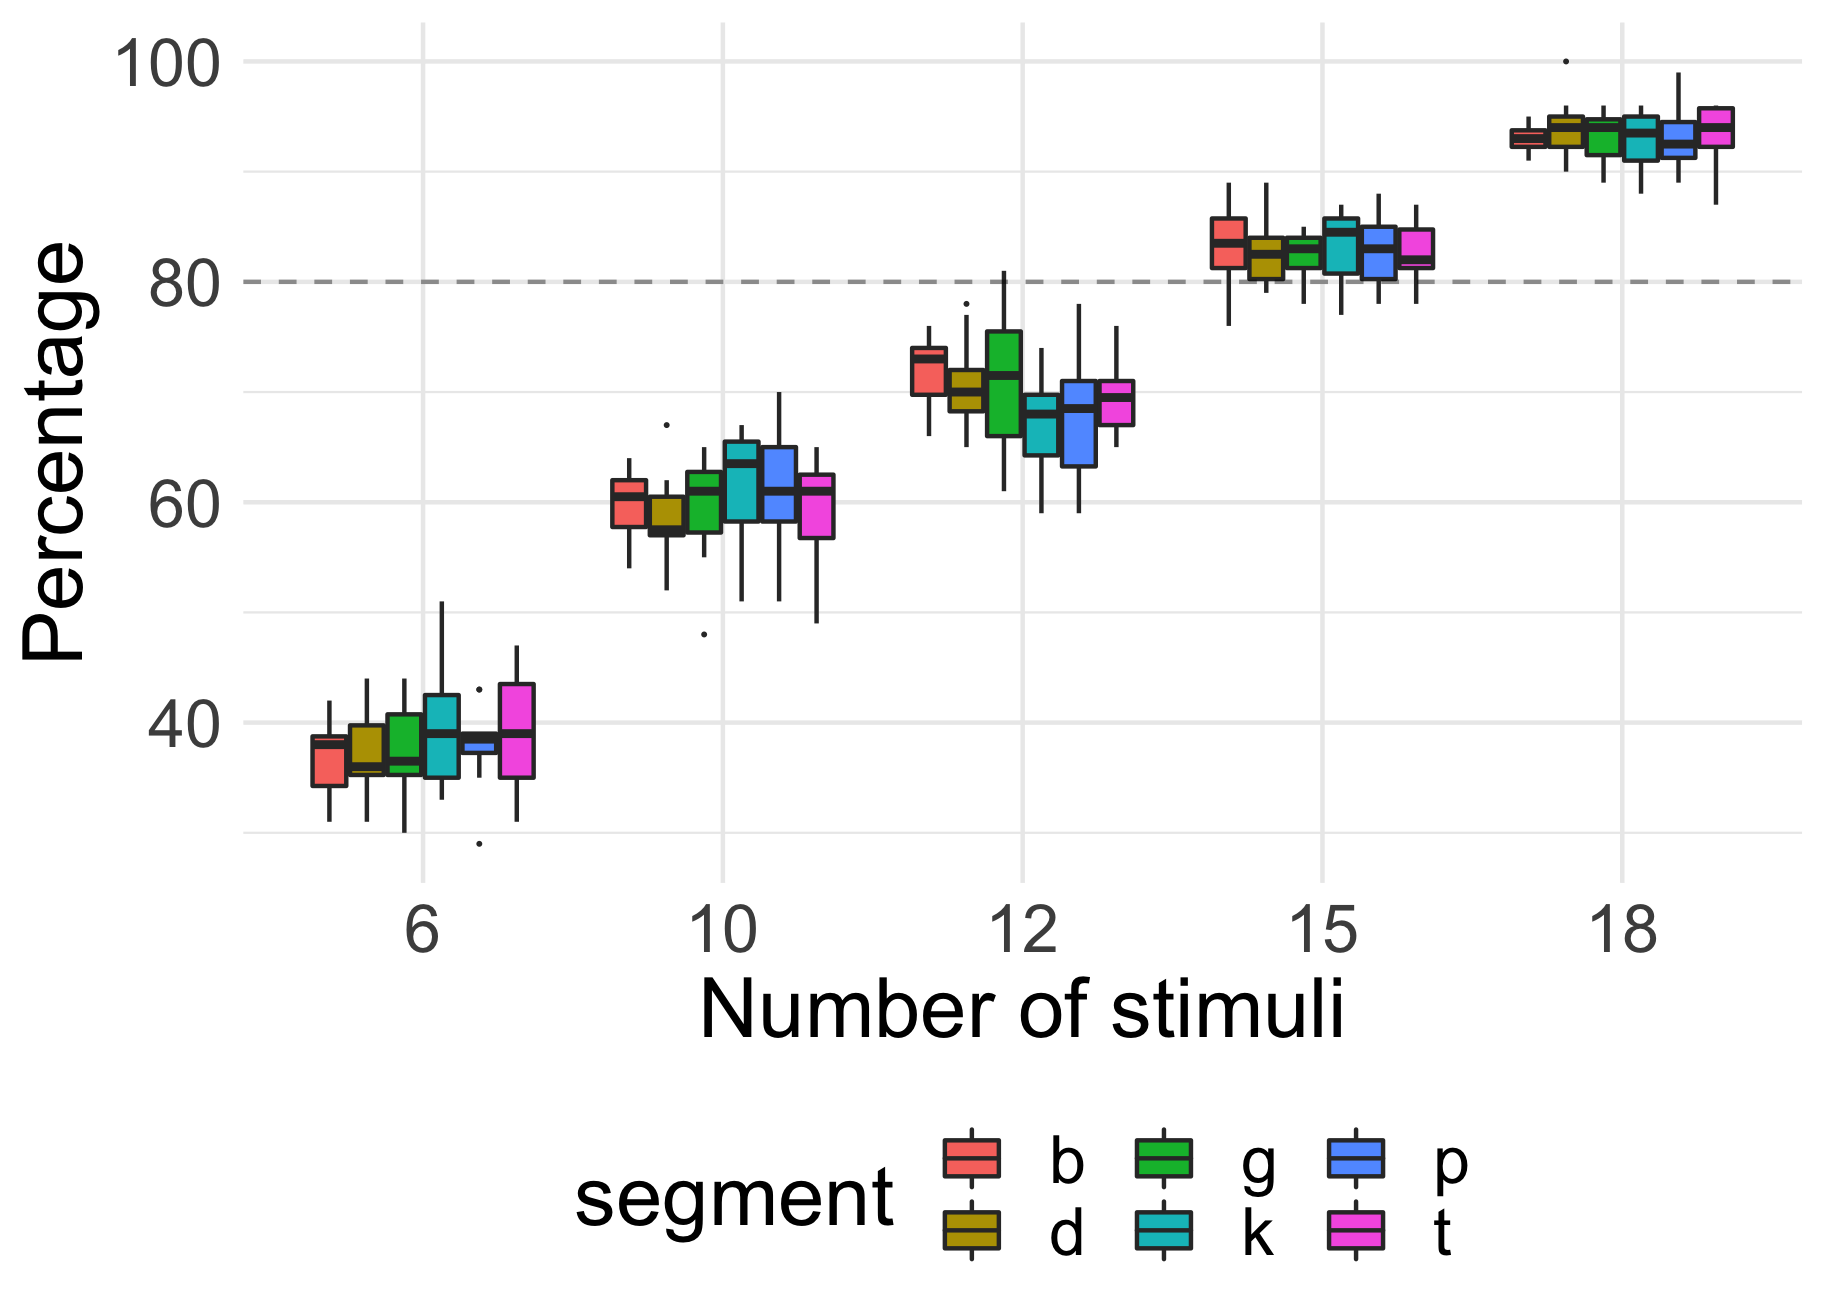
\includegraphics[width=6cm]{./includes/figures/tost.png}
  \end{center}
\end{figure}

\begin{table}[!ht]
  \caption{Percentage of significant Tests of Equivalence per sample size and segment}
  \label{tab:nums}
  \begin{center}
  \begin{tabular}{|c|c|c|c|c|c|c|}
  \hline
  \rowcolor[gray]{.75}
  n & p & t & k & b & d & g  \\
  \hline
  6 & 0.37 & 0.37 & 0.38 & 0.40 & 0.38 & 0.39 \\ 
  10 & 0.60 & 0.59 & 0.59 & 0.62 & 0.61 & 0.59 \\ 
  12 & 0.72 & 0.71 & 0.71 & 0.67 & 0.68 & 0.70 \\ 
  15 & \textbf{0.83} & \textbf{0.83} & \textbf{0.82} & \textbf{0.83} & \textbf{0.83} & \textbf{0.83} \\ 
  18 & \textbf{0.93} & \textbf{0.94} & \textbf{0.93} & \textbf{0.93} & \textbf{0.93} & \textbf{0.94} \\ 
  \hline
  \end{tabular}
  \end{center}
\end{table}

\subsection{False Positive results}

In frequentist analysis, the significance threshold (alpha - typically
.05 in linguistic research), refers to the false positive rate. That is,
when alpha is .05, it means that 5 percent of all findings would be
false positive findings, meaning that the study would report a
difference that does not actually exist. Given that our significance
threshold was .05, it is expected that around 5 percent of the total
t-tests would be positive. In total, 1455 of 30000 t-tests were
significant, or close to 5 percent. Each of these iterations also had a
significant test of equivalence, and there were 0 instances of a
significant t-test and an insignificant test of equivalence. Figure
\ref{fig:fprate} visualizes the quantity of false positive tests in the
whole data set per segment and sample size. The figure suggests that the
false positive rate does not vary much by segment or sample size, and
stays around .05. Table \ref{tab:fpos}shows the mean false positive rate
for each segment and also shows that the false positive rate ranged from
.04-.06, regardless of sample size or segment.

\begin{figure}[!ht]
  \caption{False Positive rate per sample size}
  \label{fig:fprate}
  \begin{center}
  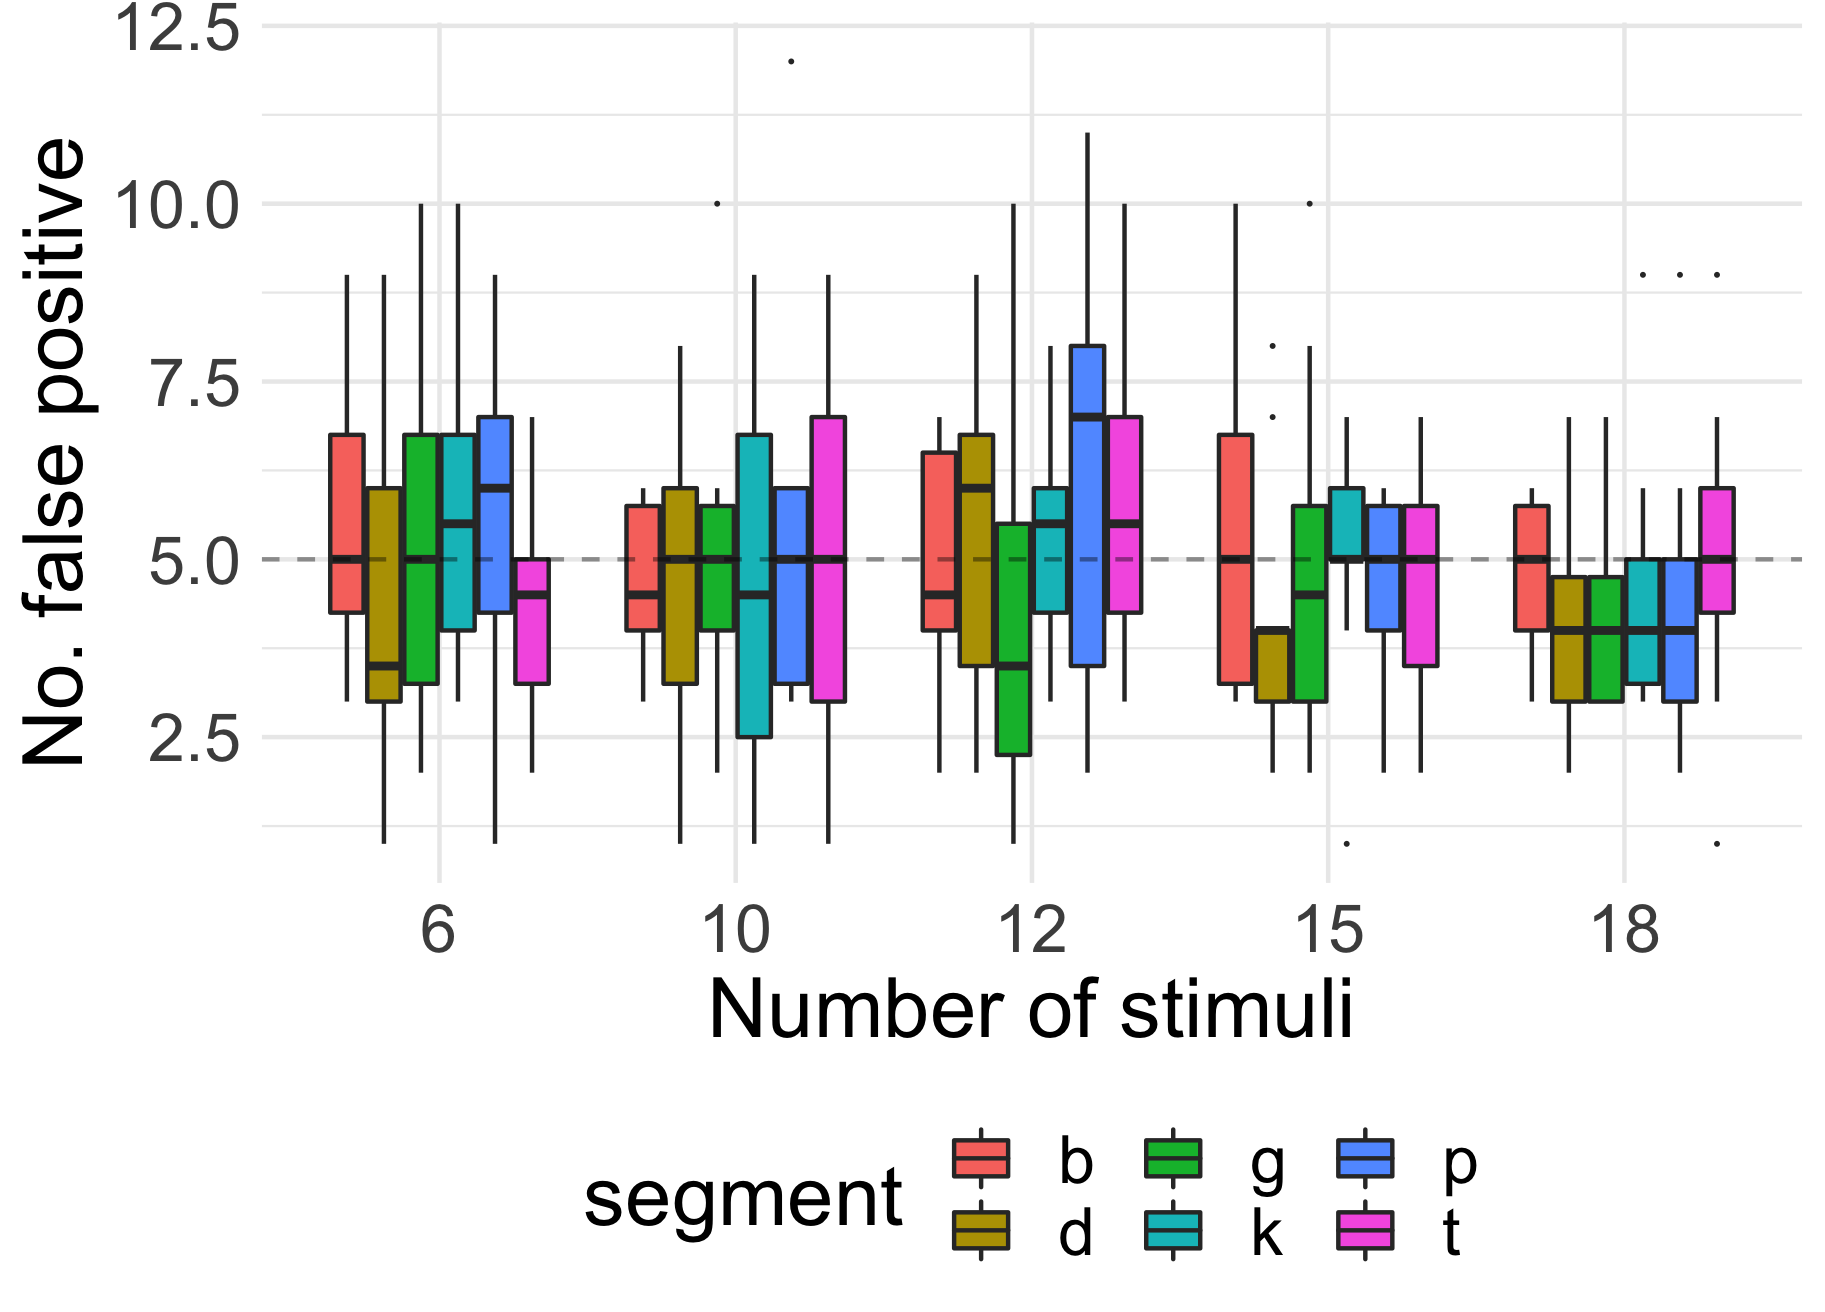
\includegraphics[width=6cm]{./includes/figures/fp_tost.png}
  \end{center}
\end{figure}

\begin{table}[!ht]
  \caption{Percentage of significant Welch's T-tests per sample size and segment}
  \label{tab:fpos}
  \begin{center}
  \begin{tabular}{|c|c|c|c|c|c|c|}
  \hline
  \rowcolor[gray]{.75}
  n & p & t & k & b & d & g  \\
  \hline
  6 & 0.06 & 0.04 & 0.05 & 0.06 & 0.06 & 0.04 \\ 
  10 & 0.05 & 0.05 & 0.05 & 0.05 & 0.05 & 0.05 \\ 
  12 & 0.05 & 0.05 & 0.04 & 0.05 & 0.06 & 0.06 \\ 
  15 & 0.06 & 0.04 & 0.05 & 0.05 & 0.05 & 0.05 \\ 
  18 & 0.05 & 0.04 & 0.04 & 0.05 & 0.04 & 0.05 \\
  \hline
  \end{tabular}
  \end{center}
\end{table}

\section{Discussion}

The results suggest that, at large, more tokens per segment should be
used in speech research, at least for VOT studies in English. These
results do not directly take into account various additional factors
which have been found to impact VOT, and it is possible that fewer
tokens might be needed in the event that there is reason to believe that
less variation exists in the underlying distribution from which an
experiment is sampling. The means and standard deviation from the
present study \cite{chodroff2017structure} included each stop 50 times
in 10 vocalic contexts, which therefore likely includes a wider range of
possible values since the following vowel has been shown to impact VOT
\cite{nearey1994effects}. This also did not account for differences in
speech rate that have been found to account for VOT
\cite{stolten2015effects}. In any case, the possible range of means and
standard deviations can be adjusted in a future analysis of repeated
measures. As a result, for VOT studies, the total of 15-18 tokens
include tokens in distinct vocalic contexts which begin with the same
segment, as long as they are balanced across conditions or languages.
For instance, if a study examines the production of word-initial /p/,
there should be 18 total words per participant which begin with /p/,
which could include 18 unique words or 6 unique words repeated 3 times
each.

In general, this study serves as an example for speech researchers to
consider how repeated measures are justified in their research, and
should be considered in tandem with the smallest effect size of
interest. For the purpose of this paper, the assumption was made that
any sample that fell within a small effect size of the underlying
distribution was practically equivalent, but this may not be a consensus
for other measures, or even in VOT for different purposes. For example,
very small effects might be taken as evidence for subtle changes in
speech such as cross-linguistic influence, studies in phonetic drift or
phonetic accommodation. In these cases, the quantity of repeated
measures may need to be increased even more for better precision.

These results provide additional context in the issues surrounding low
statistical power in not linguistic research with and emphasis on speech
research. A recent review of linguistic research at large found that
studies are typically under powered in regard to number of participants
\cite{brysbaert2021power}. That is, the low quantity of participants per
group or condition increase the probability of a false negative finding
and virtually guarantee an over-estimated effect size when an effect is
found. The finding, together with the present study, suggest that
researchers analyze how many participants are necessary and how many
tokens to elicit from each participant per condition prior to carrying
out a study. Power analysis, again, provides researchers with a
necessary tool for examining these questions.

The present study also includes open materials, including the code used
to run all analyses and to produce this manuscript. Additionally, a
shiny application was created to easily reproduce this analysis for a
single segment given a mean and standard deviation. That is, by using
the app and plugging in the mean and standard deviation, an underlying
distribution of 1000 points is created, and samples of 6, 10, 12, 15 and
18 are taken, randomly, 100 times each. A plot is then produced which
shows the number of times that each of these samples is practically
equivalent in a test of equivalence (bounds d = +/- .4). The equivalence
bounds and sample sizes can also be adjusted.

\section{Conclusion}

In conclusion, the present study has argued that more attention should
be paid to the justification of the quantity of repeated measures in
speech research. In specific, it is recommended that 18 tokens per
segment be given to a speaker in a specific condition. For example, if
one wants to study VOT of a bilingual in two languages, at least 18
tokens per segment per language would be ideal, based on the current
data. A companion shiny application was also created together with this
paper, and can be used to quickly replicate this analysis during
planning of research projects (link removed for peer review).

\bibliographystyle{./includes/bib/icphs2019.bst}
\bibliography{./includes/bib/icphs2019.bib}

\theendnotes

\end{document}
